\newcommand{\rsmpl}{\xleftarrow{\$}}

\newcommand{\alg}{\textsc{Alg}}

\newcommand{\ap}{\textsc{AccessPattern}}
\newtheorem{nonexample}[theorem]{Non-Example}


In an earlier lecture, we learned how to construct oblivious sorting, including bitonic sort which has $\mathcal{O}(n \log^2 n)$ cost~\cite{Batcher}, bucket oblivious sort~\cite{bucket} which has $\mathcal{O}(n \log n (\log \log n)^2)$ cost, 
and we showed that we can future eliminate the $(\log \log n)^2$ factor using
techniques from 
\cite{domulticore, tianyao-sort}.

We will cover Hierarchical ORAM~\cite{10.1145/233551.233553} 
in today's lecture.
Chronologically, 
Hierarchical ORAM 
was actually the original ORAM construction  
first proposed by Goldreich and Ostrovsky~\cite{10.1145/233551.233553}. 
The version we will describe in today's class
is {\it a simplified and optimized variant} of Goldreich and Ostrovsky's original
construction~\cite{10.1145/233551.233553}
introduced in Chan et al.~\cite{ohash}.
Since hierarchical ORAM consists of a hierarchy of oblivious hash tables,
let's first introduce oblivious hash table.

\section{Oblivious Hash Table}

We consider a standard static hash table abstraction.
\begin{definition}[Static Hash Table]
    Consider a data array $A = \{ (k_i, v_i) | \bot \}_{i \in [N]}$, i.e., 
each element is either a {\it real} key-value pair denoted $(k_i, v_i)$ 
or a {\it filler} denoted $\bot$. It is guaranteed that all real elements have distinct keys. An oblivious hash table contains the following operations:
    \begin{itemize}
      \item ${\sf Build}(A)$: Given a data array $A$, output a data structure.
      \item ${\sf Lookup}(k)$: Given a key $k$, output $v$. If $k = \bot$ or $k \notin A$, then output 
$v = \bot$; otherwise the output $v$ satisfies 
$(k, v) \in A$. 
    \end{itemize}

%We use the notation $(A, op)$
%to denote an operational sequence, which 
%begins with a single call to ${\sf Build}(A)$, 
%followed by a sequence of ${\sf Lookup}$s denoted $op$. 
The hash table 
we will construct satifies
obliviousnes only if the same real key
is never looked up twice. 
It turns out that such a hash table 
is sufficient for constructing hierarchical ORAM.
We now formally define this non-recurrent requirement. 
A sequence of ${\sf Lookup}$ operations denoted $op$
is said to be {\it non-recurrent} if 
every real key requested is distinct. However, the sequence  
$op$ is allowed to make filler requests $k = \bot$ multiple times. 
%that request real keys never ask for the same key
%twice.

\paragraph{Obliviousness.} Obliviousness requires the following: 
    $\forall A_0, op_0, A_1, op_1$ s.t. $|A_0| = |A_1|, |op_0| = |op_1|$ and both $op_0$ and $op_1$ satisfy the non-recurrent constraint, 
then %the oblivious hash table requires: 
it holds that 
    $$\text{AccessPattern}(A_0, op_0) \approx \text{AccessPattern}(A_1, op_1)$$
where $\text{AccessPattern}(A, op)$ denotes
the access patterns emitted
by the oblivious hash table 
when making a single call to ${\sf Build}(A)$
followed by a sequence of ${\sf Lookup}$ operations denoted $op$, 
and $\approx$ means computational indistinguishability.
More intuitively, 
we want that for any two data arrays and operation sequences of the same length, 
the access patterns in oblivious hash tables are indistinguishable as long as the same key is never looked up twice.
\end{definition}

\paragraph{Construction.}
Now let's introduce how to build an oblivious hash table.
We use the balls and bins hashing with $N$ elements (balls) and $N / Z$ 
bins\footnote{For simplicity, we assume that $N$ is divisible by $Z$.}, where $Z=\omega(\log N)$.
The expected number of elements in any fixed bin is $Z$. 
With Chernoff bound, the probability of any bin having more than $2Z$ elements is negligible in $N$.
Thus, we set the bin size to be $2Z$.
One way to randomly assign the element $(k, v)$ to a bin is to use a persudorandom function $PRF_{sk}(k)$, where the $sk$ is the secret key held by the ORAM client and the PRF output range is $[N/Z]$, indicating the desired bin index.

So now, we want to {\it obliviously} throw the balls into the bins without revealing which bin each ball goes to.
At the end, each bin is padded with filler elements to the maximum capacity.
To achieve this, we will use the 
``oblivious random bin assignment''
construction from the last lecture --- recall
from the last lecture that oblivious random bin assignment
was a key building block for constructing
an oblivious random permutation, which 
in turn served as a key building block in the construction
of bucket oblivious sort.
More specifically, the initial labels of an element with key $k$ 
is computed by $PRF_{sk}(k)$, and then we use a butterfly
network (where all intermediate bins are of size $2Z$)
to route all elements to their desired destination bins\footnote{Note that it is also possible to route the elements to bins
using oblivious sorting itself as a building block.}.
%To do this obliviously, we can use the butterfly network to route the elements to their respective bins, which is similar to the oblivious random permutation.

To implement ${\sf Lookup}(k)$, if $k$ is a real key,
the client simply reads the entire bin indexded $PRF_{sk}(k)$.
If $k = \bot$, then 
the client reads a random bin.
%So, everytime the clients lookup a fresh element, the ORAM servers will see they are accessing a random bin. In case if it's a filler element, the client will just lookup a random bin.

\paragraph{Analysis.} 
Building an oblivious hash table %involves routing elements to random bins. 
calls the ``oblivious random bin assignment'' algorithm
of the last lecture.  
Recall that in the last lecture,
we mentioned 
that using techniques from \cite{domulticore, tianyao-sort}, 
we can accomplish this with 
%Recall that in oblivious random permutation, we can accomplish this with 
$\mathcal{O}(N \log N)$ cost. %~\cite{domulticore, tianyao-sort}. 
For every lookup, the cost is the bin size, which is $Z = \omega(\log N)$.
Different from (non-oblivious) 
static hashing that has constant cost for each lookup, 
our oblivious (static) hash table has a bit higher overhead.

\section{Hierarchical ORAM}

So now with this oblivious hash table, we can construct a Hierarchical ORAM.
The hierachical ORAM essentially uses
Bentley and Saxe's hierarchical data structure idea~\cite{hierds} 
that converts
a static data structure (in our case, an oblivious hash table) 
into a dynamic one.

In Hierarchical ORAM, we have a hierarchy of exponentially growing oblivious hash tables as shown in Figure~\ref{fig:oram}.
Each level of the hierarchy has a different capacity, and the capacity grows exponentially with the level.
The levels are indexed $0, 1, \ldots, L$, and 
the $i$-th level's capacity is $2^i$.
%Level $L$ has the largest capacity $2^L$, where $L = \lceil \log N \rceil$, and 
%level $0$ has the smallest capacity $1$.
Additionally, every level has a label, either \textbf{empty} or \textbf{full}.
``Empty'' means that this level current is not being used,
and ``full'' means that 
this level is currently in use.
Whether each level is empty or full only
depends on the time step (i.e., how many operations
have been performed so far), so this information is public and
is known by the adversary.

\begin{figure}[!h]
  \centering
  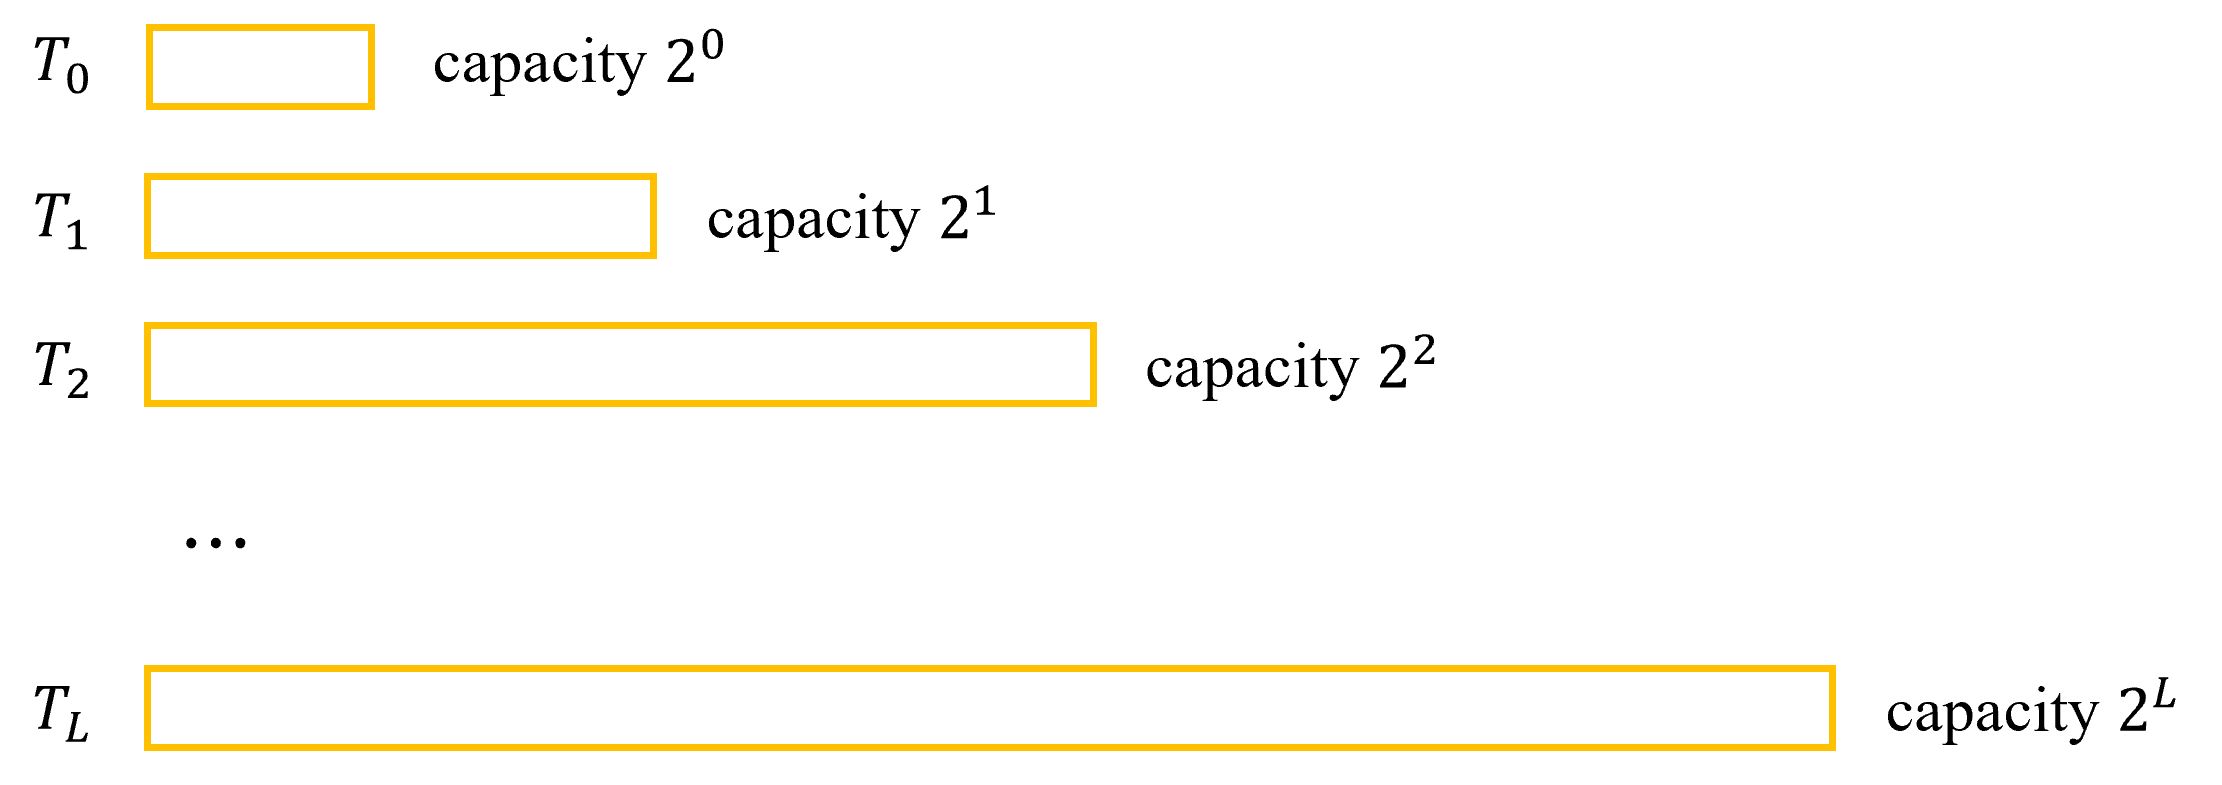
\includegraphics[width=0.8\textwidth]{fig1.png}
  \caption{Hierarchical ORAM}
  \label{fig:oram}
\end{figure}

Recall that we want to implement 
a memory abstraction with the address space $1 \ldots N$. Initially,
we may assume that all memory cells are empty and contain the symbol $\bot$. 
Therefore, initially all the ORAM levels are marked
empty.
However, later, as we perform read and write operations, at any point of time, 
some levels might be full and others are empty.

Now suppose a sequence of operations arrive.
There are two types of operations, 
%Now let's consider two operations, 
\texttt{Read}(\texttt{addr}) and \texttt{Write}(\texttt{addr}, \texttt{data}).

\paragraph{Intuition.}
Before diving into the detailed algorithm, let's first introduce the high-level idea of how to perform these operations.
%Specifically, it works as follows. 

If we want to look up some element, we will start from the smallest level.
Since every level is either empty or full. If it's full, 
look up that hash table for the desired element.
There are two outcomes: either we find the element, or we don't find the element.
If we have found the element, for all future levels, we just 
perform a fake lookup by requesting a filler element $\bot$.
Similar to the tree-based ORAM, 
we will also need to relocate the retrieved element.
So in Hierarchical ORAM, we will put the retrieved element 
to the smallest level if this level is empty.
If this level is not empty, we will need to merge the retrieved element with the existing element in this level and 
and merged hash table of size $2$ is copied to the next level
if it is empty. 
However, if the next level is not empty, then 
it causes a cascading merge until we find a level that is empty
or we reach the largest level.  
%Otherwise, if this level is still not empty, merge them again and put them to the next level, until we find the empty level to put the merged element.

\begin{algorithm}[t]
  \SetAlgorithmName{Algorithm}{algorithmautorefname}{list of algorithms name}
  \caption{\textsc{Hierarchical ORAM}}
  \label{alg:oram}
 
 \KwIn{$\texttt{addr}$, an address to lookup in the hash tables; $\texttt{op}$, the operation $\texttt{write}$ or $\texttt{read}$; $\texttt{data}$, the data to write.}
 \KwOut{$data^*$, the lookup result, if $\texttt{op} = \texttt{read}$.}
 $\texttt{found} \leftarrow false$\;
 \For{$l \leftarrow 0$ \KwTo $L$}{
   \If{not $\texttt{found}$}{
     $\texttt{fetched} \leftarrow T_l.{\sf Lookup}(\texttt{addr})$\;
     \If{$\texttt{fetched} \neq \bot$}{
        $\texttt{found} \leftarrow true$\;
        $\texttt{data}^* \leftarrow \texttt{fetched}$\;
     }
   }
   \Else{
      $T_l.lookup(\bot)$
   }
 }
 \If{$\texttt{op} = \texttt{read}$}{
  Let $T^{\phi} \leftarrow \{ (\texttt{addr}, \texttt{data}^*) \}$\;
 }
 \ElseIf{$\texttt{op} = \texttt{write}$}{
  Let $T^{\phi} \leftarrow \{ (\texttt{addr}, \texttt{data}) \}$\;
 }
 Let $l$ be the smallest level such that $T_l$ is empty, if all levels are full, let $l = L$\;
 Let $S \leftarrow T^\phi \cup T_0 \cup \cdots \cup T_{l-1}$\;
 If all levels are full, let $S \leftarrow S \cup T_L$\;
 $T_l.{\sf Build}({\sf SuppressDup}(S))$\;
 Mark $T_l$ as full, mark $T_0, \cdots, T_{l-1}$ as empty\;
 \If{$\texttt{op} = \texttt{read}$}{
  \Return{$\texttt{data}^*$}\;
 }
 \end{algorithm}



\paragraph{Algorithm.} The detailed algorithm is 
shown in Algorithm~\ref{alg:oram}. 
We use $T_0, \ldots T_L$ to denote the oblivious hash table
of the $L+1$ levels.
The algorithm starts by initiating a binary variable \texttt{found} to \texttt{false}.
Then, for each level, we check if the element is in the hash table. 
If we find the element, we set \texttt{found} to \texttt{true} and store the element in $\texttt{data}^*$.
If the element is already found, we just look up a filler 
for all future levels 
%to prevent leakage in the access patterns 
---
importantly, 
{\it this guarantees 
that the non-recurrent
constraint is satisfied for every oblivious hash table}.
After we go through all levels, 
the fetched element is in $\texttt{data}^*$.

%In the following we will do the relocate operation.
If the operation $\texttt{op}$ is \texttt{read}, we will need to write back 
the retrieved element $T^\phi = \{(\texttt{addr}, \texttt{data}^*)\}$.
Otherwise, if the operation $\texttt{op}$ is \texttt{write}, we will need to write back the new element $T^\phi = \{(\texttt{addr}, \texttt{data})\}$.
Let $l$ be the smallest level such that $T_l$ is empty, if all levels are full, let $l = L$.
We want to merge all levels $0\ldots l-1$ along with the new element 
into level $l$ (or merge all levels $0\ldots L$ along with the new
element into the largest level $L$). 
%Let $S$ be the set of elements to relocate, which is the union of the new element and all the elements in the hash tables from level $0$ to level $l-1$.
%If all levels are full, let $S$ be the union of all the elements and the new element $T^\phi$.
Then we obliviously build the hash table at level $l$ with the input set $S$.
%The build step is the same as the oblivious hash table, which is to throw the elements into the bins obliviously.
After the build step, we mark the level $l$ as 
full and the levels $0$ to $l-1$ as empty.

Note that if the oblivious hash table doesn't remove the element we just looked up, there might be duplicate elements in the set $S$ and we will need to suppress the duplicate elements.
The elements in the smaller level is always fresher than the elements in the larger level, so we can just keep the fresher element and remove the older one.
We can use the oblivious sorting to do the duplicate
suppression, denoted ${\sf SuppressDup}$
in Algorithm~\ref{alg:oram}. 
Specifically, we obliviously sort 
the elements by key and by 
freshness and removes the duplicate elements using a linear scan.


\paragraph{Analysis.} Now let's analyze the overhead of Hierarchical ORAM. 
For each request, 
there are two sources of the overhead: the lookup phase, and the rebuild phase.
The lookup cost is $L \times Z$, the number of levels $L$ times the lookup cost of at each level, which is at most the bin size $Z$.
 Recall we can set $Z = \log N \cdot \alpha(N)$, where $\alpha(N)$ is 
an arbitrarily small super-constant function. 
Thus the lookup cost is $\mathcal{O}(\log^2 N \cdot \alpha(N))$.

For rebuild cost, a level of size $2^i$ is rebuilt every $2^i$ steps.
So to rebuild a level of size $2^i$, the cost is $2^i \cdot \log 2^i$ (see the analysis of the oblivious hash table).
By amortizing the cost to each step, every level has a cost $\leq \log N$.
Thus, the rebuild cost is $\mathcal{O}(\log^2 N)$.

Summarizing the above, each memory request
has cost $\mathcal{O}(\log^2 N \cdot \alpha(N))$ where $\alpha(N)$
may be an arbitrarily small super-constant function.
Note that the original Goldreich-Ostrovsky construction~\cite{10.1145/233551.233553} has a cost of $\mathcal{O}(\log^3 N)$, because that they throw $N$ balls into $N$ bins, instead of $N/Z$ bins.



\begin{remark}
Bentley and Saxe's hierarchical data structure idea~\cite{hierds} 
is a well-known and  widely used 
technique for converting static data structures into dynamic ones,
for example, see 15451 lecture notes
(Section 2.2 in \url{https://www.cs.cmu.edu/~15451-s23/lectures/lec03-amortized.pdf}).
There has also been various applications in the cryptography literature
besides ORAM, e.g., to obtain dynamic versions of proofs 
of retrievability~\cite{dpor}, searchable encryption~\cite{dsse}, 
and private information retrieval~\cite{privblocklist}.
\end{remark}

